\section{Experiments}
\label{sec:experiments}
To fully verify the implementation of the proposed architecture, a number of experiments have been conducted. The experiments are strategically designed to test the effect of a set of features within a specific scenario. All experiments are executed in a simulated environment, from here-on called scenario. These scenarios allow us to reproduce the experiments in a controlled and predictable environment. The features were chosen in such a way that they would individually help reason about their impact on the research questions from Subsection \ref{ssec:research-questions}.

\begin{figure}[H]
    \begin{adjustwidth}{-2cm}{}
        \centering
        % \begin{table}[]
        \begin{tabular}{l|llll}
            \textbf{Features \textbackslash Scenarios} & \textbf{No interaction} & \textbf{Growing Infrastructure} & \textbf{Unstable Infrastructure} & \textbf{Mixed} \\ \hline
            \textbf{Local}                             & A.1            & A.2                    & A.3                     & A.4   \\
            \textbf{Knowledge-Sharing only}            & B.1            & B.2                    & B.3                     & B.4   \\
            \textbf{Auctioning}                        & C.1            & C.2                    & C.3                     & C.4     
        \end{tabular}
        \caption{\label{fig:experiments}Overview of the experiments that are conducted. Each scenario is conducted with a different set of features, to test the effect of the features on the results.}
        % \end{table}
    \end{adjustwidth}
\end{figure}

\subsection*{Features}


\begin{figure}[H]
    % \begin{table}[]
        \centering
        \begin{tabular}{l|l|l|l}
            \textbf{Feature \textbackslash Name} & \textbf{Local} & \textbf{Knowledge-Sharing} & \textbf{Auctioning} \\ \hline
            \textbf{Inspect host properties}     & yes            & yes                        & yes                 \\
            \textbf{Adapt host properties}       & yes            & yes                        & yes                 \\
            \textbf{Risk analysis}               & yes            & yes                        & yes                 \\
            \textbf{Share knowledge}             & no             & yes                        & yes                 \\
            \textbf{Initiate \& Join auctions}   & no             & no                         & yes                 \\
            \textbf{Migrate Software}            & no             & no                         & yes                            
        \end{tabular}
        \caption{\label{fig:experiment-features}Overview of the actions that are allowed in each feature set. }
    % \end{table}
\end{figure}

\begin{description}
    \item[Local*]             Agents are able to inspect, and adapt their own properties and software components. They are also allowed to do risk analysis on their knowledge base. 
    \item[Knowledge-Sharing*] Agents are able to do all of the above, and they are able to share knowledge with other agents to update their own knowledge base.
    \item[Auctioning]         Agents are able to do all of the above, and they are able to cooperate with other agents to mitigate risks through auctions. Only in this stage are agents able to join and initiate auctions.
\end{description}

{\small \textit{*The adaptations at this point only include the ability to make attribute changes. Software migrations are excluded as an agent has insufficient knowledge and capabilities to perform the migration to a node that is not its own.}}

\subsection*{Scenarios}
As mentioned before, each of the feature sets are executed in a specific scenario. A scenario is defined by an infrastructure and a set of events that will happen over time. These events could be new nodes joining the infrastructure, or nodes leaving the infrastructure. Because of the scenarios it was possible to repeat the experiments over-and-over again without having to manually change the infrastructure. This allowed for better reason about and compare the results of each individual experiment. Additionally it allowed for a more realistic approach to the experiments, as the infrastructure is not static and is changing over time.

Four scenarios have been defined, each with a different set of characteristics. These characteristics are defined as follows:

\begin{description}
    \item[No interaction]             No infrastructure changes are made overtime.
    \item[Growing Infrastructure]     The infrastructure is slowly growing over time.
    \item[Unstable Infrastructure]    Some nodes in the infrastructure are unstable and are disconnected from the network from time to time.
    \item[Mixed]                      A more realistic scenario where nodes are added and removed from the infrastructure over time.
\end{description}


% The experiments are conducted in a simulated environment, where the agents are connected to a \code{ExperimentManager} which is responsible for creating the infrastructure, \comment{Zoltan}{is this really done by the ExperimentManager}managing the communication between agents, starting the experiment, and stopping the experiment after a predefined number of epochs\footnote{Epochs are further explained in REFERENCE}. The \code{ExperimentManager} is also responsible for measuring metrics as explained in Section \ref{ssec:metrics}. \comment{Zoltan}{I think that shouldn't matter}The experiments are conducted in the following order:

% \begin{enumerate}
%     \item Baseline experiment
%     \item Experiment 1: Risk Analysis 
%     \item Experiment 2: Risk Mitigation 
% \end{enumerate}

% \comment{Zoltan}{It's worth emphasizing that the experiments are conducted in a simulated environment.}
% Each of the experiments is performed on the same infrastructure, but with different configurations. \tocheck{Update this depending on the final infrastructure} The infrastructure is a simple network consisting of 4 nodes, where each node has 4 software components. The nodes are connected as shown in Figure \ref{fig:infrastructure}. The infrastructure is created by the \code{ExperimentManager} and is the same for all experiments.

% \begin{figure}[H]
%     \centering
%     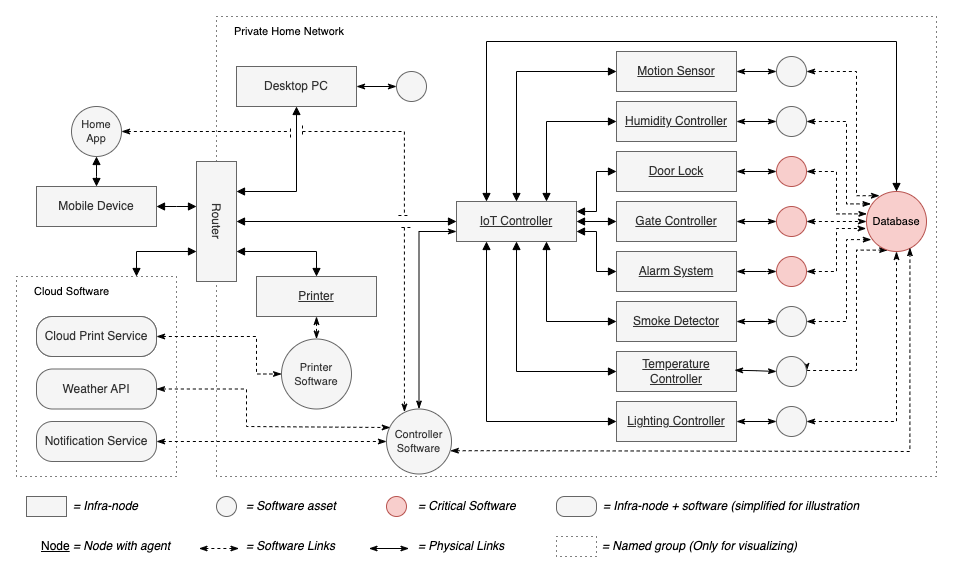
\includegraphics[width=0.8\textwidth]{_content/infrastructure}
%     \caption{Experiment Infrastructure.}
%     \label{fig:infrastructure}
% \end{figure}
% \comment{Zoltan}{What do the arrows mean? I think they might have different meaning, depending on whether they connect two nodes or a node and a SW Component}

\subsection{Metrics and Evaluation}
\label{ssec:metrics}

% As mentioned above the \code{ExperimentManager} is responsible for measuring metrics. These metrics are measured for each epoch, and is repeated for each experiment. 
% \comment{Zoltan}{Idea: These metrics could be categorized as effectiveness metrics and efficiency metrics. The first and the last measure efficiency, while the others measure effectiveness.}

\begin{figure}[H]
    \centering
    \begin{tabular}{l|l}
        \textbf{Effectiveness}            & \textbf{Efficiency}            \\ \hline
        Total \# of risk identified       & Total \# of messages exchanged \\
        \# of remaining risks             & \# of adaptations              \\
        Weighted damage of remaining risk &                               
    \end{tabular}
    \caption{\label{fig:metrics-groups}Overview of the metrics that are measured, grouped by their category.}
\end{figure}


The metrics are defined as follows:

\begin{description}
    \item[Total number of messages exchanged] The total number of messages exchanged between agents during the epoch.
    \item[Total number of risks identified] The total number of risks identified by the agents during the epoch.
    \item[Number of remaining risks] The number of risks that have not been mitigated by the agents during the epoch.
    \item[Sum of the damage for remaining risks] The sum of the damage for the risks that have not been mitigated by the agents during the epoch.
    \comment{Zoltan}{I think this should be weighted by the probability of those risks}
    \item[Number of adaptations] The number of adaptations performed by the agents during the epoch.
\end{description}

\subsection{Controls and Variables}
\label{ssec:controls-variables}
\begin{quote}\textcolor{red}{
    Discuss any controls or variables that were taken into account to ensure the validity and reliability of your results. This could include experimental controls, randomization, and addressing potential confounding factors.
}\end{quote}

% \subsection{Baseline Experiment}
% % - No communication, no cooperation
% % - Predefined Infrastructure, same as other experiments
% % - Measure:
% %   - Number of adaptations
% %   - Total number of risks identified
% %   - Number of remaining risks
% %   - Sum of the damage for remaining risks

% % Mitigations take time, also communication. This should be discussed and used in the experiment.
% % Check costs of a mitigation

% \comment{Zoltan}{Arent these metrics collected in all experiments}The baseline experiment is conducted to measure metrics such as the number of adaptations and the number of risks identified. In this experiment Agents are not able to communicate with each other, and are not able to cooperate. 

% When the experiment has started, the agents are allowed to adapt their own properties and software components. However, the agents are not able to share knowledge and otherwise communicate with each other. To make the experiment easier to manage the \code{ExperimentManager} still is able to send messages to the agents, but the agents are not able to send messages to each other. \comment{Zoltan}{and also not able to cooperatively discover risks that require a global view I guess} Agents to being able to cooperate means that they are not able to join in auctions and therefore not able to work together to mitigate risks. A schematic overview of the experiment is shown in Figure \ref{fig:baseline}.

% \begin{figure}[H]
%     \centering
%     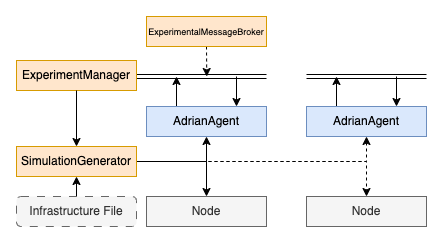
\includegraphics[width=0.8\textwidth]{_content/adrian-experiment-0}
%     \caption{Schematic overview of the baseline experiment, where multiple Agents are disconnected from one another.}
%     \label{fig:baseline}
% \end{figure}
% \comment{Zoltan}{It's not fully clear what this figure conveys. What do the individual symbols mean? In general, it is a good idea to explain all figures in the text, because they are often not as self-explanatory as you might think.}

% \subsection{Experiment 1: Risk Analysis}
% % - Communication, no cooperation
% % - Predefined Infrastructure, same as other experiments
% % - Measure:
% %   - Number of adaptations
% %   - Total number of messages exchanged
% %   - Total number of risks identified
% %   - Number of remaining risks
% %   - Sum of the damage for remaining risks

% The first experiment is conducted to measure the effect of communication between agents. In this experiment agents are able to communicate with each other, \comment{Zoltan}{I think you mean this only for mitigation, not for risk identification?} but are not able to cooperate. 

% When the experiment has started, the agents are allowed to adapt their own properties and software components. The agents are also able to share knowledge at a distance of \( D_{knowledge} \). In this experiment Agents are still not able to cooperate on mitigating risks, which is achieved by not allowing Agents to initiate or join auctions. A simplified overview of the experiment is shown in Figure \ref{fig:experiment-1}.

% \begin{figure}[H]
%     \centering
%     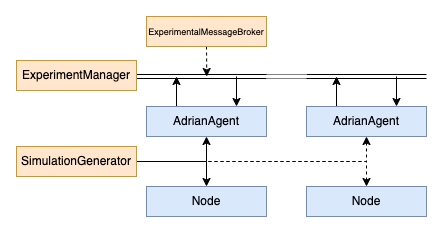
\includegraphics[width=0.8\textwidth]{_content/adrian-experiment-1}
%     \caption{Schematic overview of the first and second experiment, depicting the way multiple Agents are connected to each other and are controlled by the \code{ExperimentManager}.}
%     \label{fig:experiment-1}
% \end{figure}
% \comment{Zoltan}{It's not easy to spot the difference between this and the previous figure, like in a puzzle. Please make the life of your readers easier.}

% This experiment is repeated multiple times, with different values for \( D_{knowledge} \). The values for \( D_{knowledge} \) are 1, 2, and 3. The results of this experiment are compared to the results of the baseline experiment.

% \subsection{Experiment 2: Risk Mitigation}
% % - Communication, cooperation
% % - Predefined Infrastructure, same as other experiments
% % - Measure:
% %   - Number of adaptations
% %   - Total number of messages exchanged
% %   - Total number of risks identified
% %   - Number of remaining risks
% %   - Sum of the damage for remaining risks

% The second experiment is conducted to measure the effect of cooperation between agents. In this experiment agents are able to communicate with each other, and are able to cooperate. 

% When the experiment has started, the agents are allowed to adapt their own properties and software components. The agents are also able to share knowledge at a distance of \( D_{knowledge} \). Additionally, in this experiment Agents are able to cooperate on mitigating risks, which is achieved by allowing Agents to initiate and join auctions. The overview of this experiment is shown in Figure \ref{fig:experiment-1}.

% As with the first experiment, this experiment is repeated multiple times, with different values for \( D_{knowledge} \). The values for \( D_{knowledge} \) are 1, 2, and 3. The results of this experiment are compared to the results of the baseline experiment and the first experiment.
